\documentclass[11pt,a4paper]{report}%especifica o tipo de documento que tenciona escrever: carta, artigo, relatório... neste caso é um relatório
% [11pt,a4paper] Define o tamanho principal das letras do documento. caso não especifique uma delas, é assumido 10pt
% a4paper -- Define o tamanho do papel.
\usepackage{float}
\usepackage[portuges]{babel}%Babel -- irá activar automaticamente as regras apropriadas de hifenização para a língua todo o
                                   %-- o texto gerado é automaticamente traduzido para Português.
                                   %  Por exemplo, “chapter” irá passar a “capítulo”, “table of contents” a “conteúdo”.
                                   % portuges -- específica para o Português.
\usepackage[utf8]{inputenc} % define o encoding usado texto fonte (input)--usual "utf8" ou "latin1

\usepackage{graphicx} %permite incluir graficos, tabelas, figuras
\usepackage{url} % para utilizar o comando \url{}
\usepackage{enumerate} %permite escolher, nas listas enumeradas, se os iems sao marcados com letras ou numeros-romanos em vez de numeracao normal

%\usepackage{apalike} % gerar biliografia no estilo 'named' (apalike)

\usepackage{color} % Para escrever em cores
\usepackage{multirow} %tabelas com multilinhas
\usepackage{array} %formatação especial de tabelas em array

\usepackage[pdftex]{hyperref} % transformar as referências internas do seu documento em hiper-ligações.

%Exemplos de fontes -- nao e vulgar mudar o tipo de fonte
%\usepackage{tgbonum} % Fonte de letra: TEX Gyre Bonum
%\usepackage{lmodern} % Fonte de letra: Latin Modern Sans Serif
%\usepackage{helvet}  % Fonte de letra: Helvetica
%\usepackage{charter} % Fonte de letra:Charter

\definecolor{saddlebrown}{rgb}{0.55, 0.27, 0.07} % para definir uma nova cor, neste caso 'saddlebrown'

\usepackage{listings}  % para utilizar blocos de texto verbatim no estilo 'listings'
%paramerização mais vulgar dos blocos LISTING - GENERAL
\lstset{
	basicstyle=\small, %o tamanho das fontes que são usadas para o código
	numbers=left, % onde colocar a numeração da linha
	numberstyle=\tiny, %o tamanho das fontes que são usadas para a numeração da linha
	numbersep=5pt, %distancia entre a numeração da linha e o codigo
	breaklines=true, %define quebra automática de linha
    frame=tB,  % caixa a volta do codigo
	mathescape=true, %habilita o modo matemático
	escapeinside={(*@}{@*)} % se escrever isto  aceita tudo o que esta dentro das marcas e nao altera
}
%
%\lstset{ %
%	language=Java,							% choose the language of the code
%	basicstyle=\ttfamily\footnotesize,		% the size of the fonts that are used for the code
%	keywordstyle=\bfseries,					% set the keyword style
%	%numbers=left,							% where to put the line-numbers
%	numberstyle=\scriptsize,				% the size of the fonts that are used for the line-numbers
%	stepnumber=2,							% the step between two line-numbers. If it's 1 each line
%											% will be numbered
%	numbersep=5pt,							% how far the line-numbers are from the code
%	backgroundcolor=\color{white},			% choose the background color. You must add \usepackage{color}
%	showspaces=false,						% show spaces adding particular underscores
%	showstringspaces=false,					% underline spaces within strings
%	showtabs=false,							% show tabs within strings adding particular underscores
%	frame=none,								% adds a frame around the code
%	%abovecaptionskip=-.8em,
%	%belowcaptionskip=.7em,
%	tabsize=2,								% sets default tabsize to 2 spaces
%	captionpos=b,							% sets the caption-position to bottom
%	breaklines=true,						% sets automatic line breaking
%	breakatwhitespace=false,				% sets if automatic breaks should only happen at whitespace
%	title=\lstname,							% show the filename of files included with \lstinputlisting;
%											% also try caption instead of title
%	escapeinside={\%*}{*)},					% if you want to add a comment within your code
%	morekeywords={*,...}					% if you want to add more keywords to the set
%}

\usepackage{xspace} % deteta se a seguir a palavra tem uma palavra ou um sinal de pontuaçao se tiver uma palavra da espaço, se for um sinal de pontuaçao nao da espaço

\parindent=0pt %espaço a deixar para fazer a  indentação da primeira linha após um parágrafo
\parskip=2pt % espaço entre o parágrafo e o texto anterior

\setlength{\oddsidemargin}{-1cm} %espaço entre o texto e a margem
\setlength{\textwidth}{18cm} %Comprimento do texto na pagina
\setlength{\headsep}{-1cm} %espaço entre o texto e o cabeçalho
\setlength{\textheight}{23cm} %altura do texto na pagina

% comando '\def' usado para definir abreviatura (macros)
% o primeiro argumento é o nome do novo comando e o segundo entre chavetas é o texto original, ou sequência de controle, para que expande
\def\darius{\textsf{Darius}\xspace}
\def\antlr{\texttt{AnTLR}\xspace}
\def\pe{\emph{Publicação Eletrónica}\xspace}
\def\titulo#1{\section{#1}}    %no corpo do documento usa-se na forma '\titulo{MEU TITULO}'
\def\super#1{{\em Supervisor: #1}\\ }
\def\area#1{{\em \'{A}rea: #1}\\[0.2cm]}
\def\resumo{\underline{Resumo}:\\ }

%\input{LPgeneralDefintions} %permite ler de um ficheiro de texto externo mais definições

\title{Projeto de System Deployment \& Benchmarking\\
       \textbf{Instalação Zulip}\\ Relatório de Desenvolvimento
       } %Titulo do documento
%\title{Um Exemplo de Artigo em \LaTeX}
\author{José André Martins Pereira\\ (a82880@alunos.uminho.pt) \and Ricardo André Gomes Petronilho\\ (a81744@alunos.uminho.pt) \and Miguel Raposo Dias\\ (pg41089@alunos.uminho.pt) \and
Ricardo Cunha Dias \\ (pg39295@alunos.uminho.pt)
       } %autores do documento
\date{\today} %data

\usepackage{hyperref}
\hypersetup{
    colorlinks=true,
    linkcolor=blue,
    filecolor=magenta,      
    urlcolor=blue,
}
 
\urlstyle{same}

\begin{document} % corpo do documento
\maketitle % apresentar titulo, autor e data

\begin{abstract}  % resumo do documento
Na Unidade Curricular de Systems Deployment \& Benchmarking foi-nos proposta a elaboração de um projeto de análise e deployment da aplicação Zulip, bem como a interpertação da arquitetura da mesma.
\end{abstract}

\tableofcontents % Insere a tabela de indice
%\listoffigures % Insere a tabela de indice figuras
%\listoftables % Insere a tabela de indice tabelas

\chapter{Introdução} \label{chap:intro} %referência cruzada
Na unidade curricular de \textbf{Systems Deployment \& Benchmarking} foi-nos proposto um trabalho prático de análise, deployment e benchmarking de uma aplicação.\\

A aplicação escolhida pela equipa foi o \textbf{\href{https://zulipchat.com}{Zulip}}, na medida em que segue os requisitos do trabalho prático, bem como, tem uma boa documentação.
O \textbf{Zulip} é uma aplicação de chat em tempo real, onde o principal objetivo é oferecer um boa experiência a organizações, empresas e projetos voluntários, de pequenas equipas de amigos, até dezenas de milhares de utilizadores.\\

O objetivo principal deste trabalho prático é perceber a arquitetura da aplicação, deployment/instalação da mesma e respetivas configurações, as formas de comunicação entre os diferentes componentes e por fim a identificação de operações onde o desempenho seja crítico.


\chapter{Arquitetura}

\section{Especificação}

\begin{figure}[H]
	\centering
	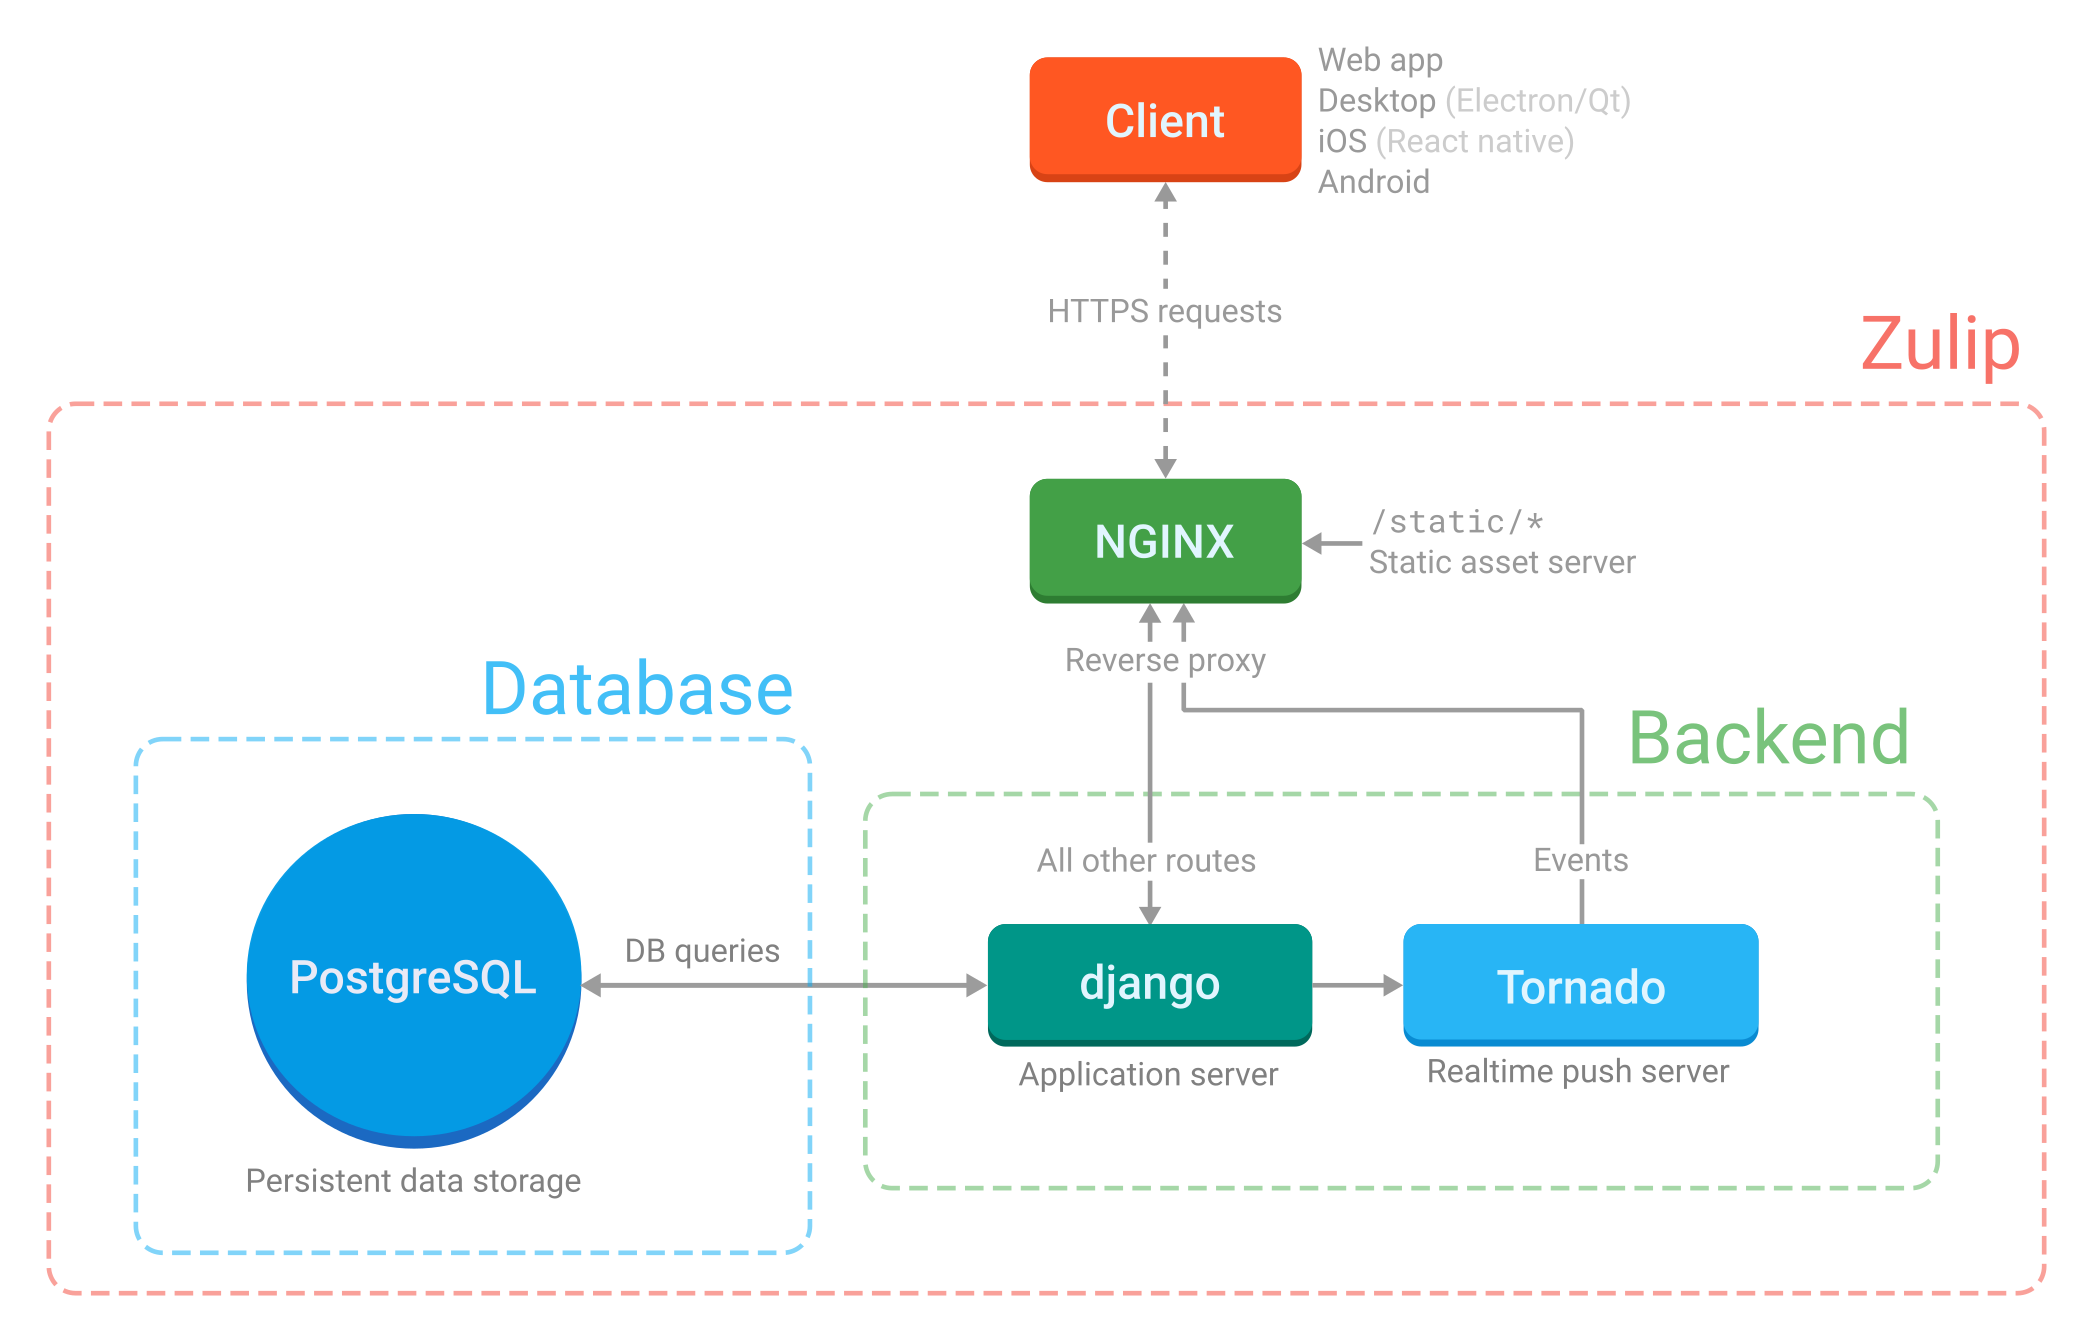
\includegraphics[scale=0.28]{architecture.png}
	\caption{\href{https://zulip.readthedocs.io/en/latest/overview/architecture-overview.html}{Arquitetura da aplicação Zulip.}}
	\label{img:arquitetura-zulip}
\end{figure}

A arquitetura da aplicação \textbf{zulip} contém vários \textbf{componentes}, sendo que, se consegue dividir os mesmos em diferentes subsistemas. No entanto, é perceptível pela figura \ref{img:arquitetura-zulip}, que existe uma separação entre o componente \textbf{Client} com os restantes, pois são subsistemas distintos.
\newline
O \textbf{Client} é responsável pela apresentação (\emph{view}) da aplicação, enquanto que o restante subsistema é de uma forma geral, responsável pela lógica e tratamento de dados da mesma, sendo este mais complexo e composto por subsistemas interiores (\textbf{Database} \& \textbf{Backend}).
\newline
A divisão também deve-se ao facto do componente \textbf{Client} estar na máquina do utilizador, enquanto que os restantes estarão em máquinas administradas pela empresa de desenvolvimento.
\newline
O componente \textbf{NGINX} consiste num servidor \emph{HTTP} intermediário (\emph{middleware}) entre o componente \textbf{Client} com \emph{HTTP requests} e o \textbf{Backend}. Na verdade, o \textbf{NGINX} permite uma independência entre os subsistemas, ou seja, o \textbf{Client}, pode ser definido para diferentes plataformas, nomeadamente: web, desktop, iOS e android.
\newline
Em relação à base de dados da aplicação, tem-se o componente \textbf{PostgreSQL}, um sistema de gerenciamento de dados persistente que apenas comunica com o servidor da aplicação \textbf{django}.
\newline
Em termos do sistema de \textbf{backend} da aplicação, este é composto por duas componentes, sendo elas \textbf{django} e \textbf{Tornado}, este primeiro \textbf{django} é de extrema importância tendo em conta que é a base da construção da aplicação \textbf{zulip}, e consiste num framework de web do lado do servidor de código aberto, desenvolvido em Python, fornecendo assim todo o framework necessário para ser mais tarde apresentado do lado do cliente, quanto ao \textbf{Tornado} é um servidor de web assíncrono e sem bloqueio de I/o que permite manter ativas milhares de ligações em tempo real, no caso do \textbf{zulip} é respónsavel pela entrega de mensagens e não muito mais.\\ Outros componentes secundários igualmente importantes no funcionamento do \textbf{zulip} são \textbf{Supervisor} que é um sistema cliente/servidor que permite monitorizar e controlar os processos em sistemas \textbf{unix}, no caso do \textbf{zulip} é utilizado para iniciar os processos do servidor, reinicializar-los em caso de falha e fazer \emph{logging}, outro é \textbf{memcached} é um sistema distribuído de cache em memória, é usado para guardar em chache modelos de dados e invalidar-los caso sejam alterados.\\
Um outro componente secundário é a base de dados em memória \textbf{Redis} que armazena chaves com durabilidade opcional, é usado para guardar dados com tempo de vida bastante baixo.\\ O \textbf{RabbitMQ} é um software de mensagens com código aberto, que é usado para tratar de filas que requerem uma entrega fiável mas não são passíveis de fazer no sistema principal, é também usado para comunicações entre \textbf{django} e \textbf{Tornado}.\\ Por último, o componente \textbf{Thumbor} é um serviço de miniaturas de fotos open-source que tem como função administrar as fotos do sistemas ora via \textbf{upload} ora via \textbf{url}. 


\chapter{Padrões de distribuição e comunicação}

A aplicação apresenta dois padrões bem definidos, nomeadamente o padrão \textbf{Cliente-Servidor} de onde advem a sua arquitera e o padrão \textbf{\textit{Brooker}} usado na comunicação do componente \textbf{RabbitMQ} e serviços conectados a ele.

\section{Padrão Cliente-Servidor}

Este padrão consiste em duas partes. O servidor que fornece diferentes serviços e o cliente que os consome. A comunicação entre as duas partes, \textbf{Cliente} (aplicação móvel, web ou nativa) e \textbf{Servidor} (NGINX), é feita através do protocolo \textbf{HTTP}.

\begin{figure}[H]
	\centering
	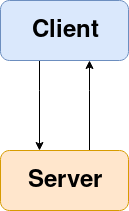
\includegraphics[scale=0.50]{client_server.png}
	\caption{Padrão Cliente-Servidor}
	\label{img:cliente-servidor}
\end{figure}

\section{Padrão \textit{Brooker}}

Este padrão é utilizado na comunição de componentes independentes entre eles. A comunicação entre estes componentes é feita através de "mensagens" (\textbf{AMQP}) enviadas pelos componentes, as quais são depois recebidas pelo intermediário (\textbf{RabbitMQ}) que é responsável pela distribuição das mensagens pelo outros componentes. 

\begin{figure}[H]
	\centering
	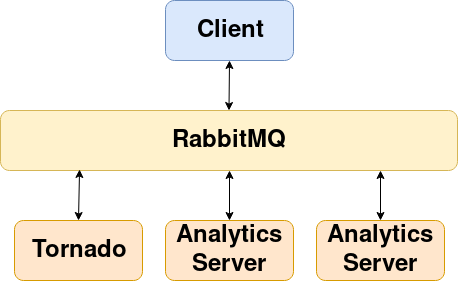
\includegraphics[scale=0.50]{broker.png}
	\caption{Padrão \textit{Brooker}}
	\label{img:brooker}
\end{figure}

\chapter{Configuração}

Os vários requisitos para correr o servidor Zulip estão detalhados na \href{https://zulip.readthedocs.io/en/latest/production/requirements.html}{documentação oficial}, vamos apenas especificar a configuração utilizada pelo nosso grupo.

\section{Instalação}

Tal como nas aulas práticas utilizou-se o \textbf{Virtual Box} criando um \textbf{Vagrantfile} com a configuração, desta forma a instalação é totalmente automática.

O sistema operativo é o  \textbf{Ubuntu Xenial 16.04}, o hardware simulado tem  \textbf{2 GB de RAM} e  \textbf{2 CPUs} dedicados. 

O endereço IP é estático: \textbf{10.0.0.101}. Para que outras máquinas externas ao host consigam ter acesso ao servidor instalado na VM recorreu-se à abertura das portas (\textbf{portforward}):  \textbf{80} e  \textbf{443}; estas são responsáveis pelo protocolo HTTP e HTTPS respetivamente. A seguinte figura ilustra a implementação deste passo:

\begin{figure}[H]
	\centering
	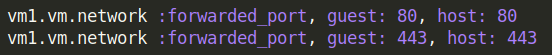
\includegraphics[scale=0.6]{portfoward.png}
	\caption{Portfoward das portas 80 e 443.}
	\label{img:pag}
\end{figure}

Apesar da documentação oficial recomendar, \textbf{não se configurou um endereço DNS} uma vez que o ambiente é apenas de teste.
O servidor zulip obriga o uso de um \textbf{certificado SSL}, pelo motivo referido anteriormente, foi gerado um \textbf{auto-certificado}. No entanto, por questões de segurança o Google Chrome e outros browsers por padrão não permitem o acesso a páginas com auto-certificados SSL ou desatualizados, desta forma foi necessário ativar essa funcionalidade acedendo (no Chrome) à página: \url{chrome://flags/} tal como a figura mostra: 

\begin{figure}[H]
	\centering
	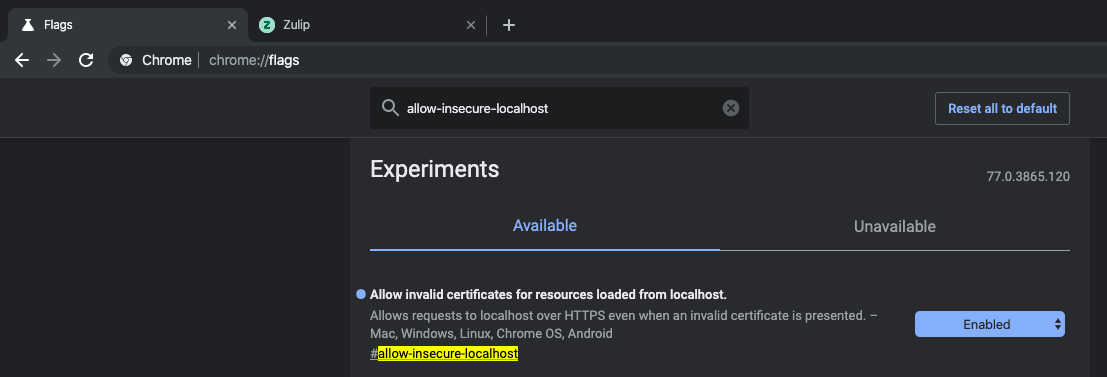
\includegraphics[scale=0.35]{allow_ssl_localhost.png}
	\caption{Ativação de páginas com auto-certificados SSL no Google Chrome.}
	\label{img:pag}
\end{figure}

Finalmente para instalar o servidor apenas é necessário correr os seguintes comandos, estando os mesmos no Vagrantfile para uma instalação automática.

\begin{figure}[H]
	\centering
	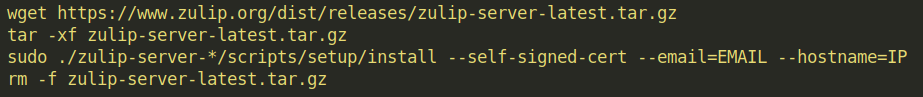
\includegraphics[scale=0.5]{install_zulip.png}
	\caption{Label.}
	\label{img:pag}
\end{figure}

O \textbf{wget} descarrega os ficheiros necessários à instalação, o \textbf{tar} descompacta-os, \textbf{sudo ./...} corre o instalador, note-se que se usa \textbf{.*} na versão do instalador tornando o comando único/ genérico para qualquer versão e, finalmente, o \textbf{rm} elemina os ficheiros do instalador uma vez que já não são necessários.

No argumento \textbf{--email} deve ser referido o email de administrador que recebe mensagens de erros e suporte. O \textbf{--hostname} é o endereço utilizado para aceder ao servidor, no nosso caso é um endereço IP mas podia ser um endereço DNS. Tal como referido anteriormente o argumento \textbf{--sel-signed-cert} gera um auto-certificado SSL. Estes argumentos podem ser novamente configurados após a instalação.


\newpage 
\section{Servidor email}

\subsection{Outgoing email}

Após a instalação deve ser configurado um servidor \textbf{SMTP} - \textbf{S}imple \textbf{M}ail \textbf{T}ransfer \textbf{P}rotocol - uma vez que o servidor zulip necessita de enviar emails para os utilizadores para confirmação de contas, notificações, entre outros. 

É possível instalar o servidor SMTP na mesma máquina (localhost) em que o servidor zulip se encontra, a equipa preferiu usar um servidor remoto já configurado. Como o ambiente de instalação é apenas de teste, recorreu-se a um servidor SMTP falso, isto é, um servidor que em vez de realmente enviar emails aos utilizadores, os mesmos ficam retidos sendo apenas uma simulação de envio, utilizando para isso o \href{https://mailtrap.io/}{mailtrap}.

No ficheiro \textbf{/etc/zulip/settings.py} é possível configurar o servidor SMTP, para tal devem ser definidas as seguintes variáveis:

\begin{itemize}
    \item EMAIL\_HOST
    \item EMAIL\_HOST\_USER
    \item EMAIL\_PORT
\end{itemize}

Por último no ficheiro \textbf{/etc/zulip/zulip-secrets.conf} define-se a password do servidor na variável \newline \textbf{email\_password}.

Após a configuração é necessário reiniciar o zulip atavés do seguinte comando: 

\textbf{sudo su zulip -c '/home/zulip/deployments/current/scripts/restart-server'}

Desta forma todos os serviços e componentes associados ao servidor zulip são reiniciados.


\subsection{incoming email}

O incoming email, permite enviar mensagens  para o \textbf{zulip} via email, garantindo assim integrar aplicações de terceiros para enviar mensagens ("notificações") para o \textbf{zulip} e os utilizadores poderem responder a emails de notificações.\newline Existem duas formas de configurar o gateway de email:
\\

\begin{itemize}
    \item \textbf{Localmente}: um servidor \textbf{Postfix} corre no servidor e direciona as mensagens diretamente para a aplicação.
    \item \textbf{Polling}: uma tarefa agendada(\textbf{cron job}) que corre na aplicação que verifica minuto a minuto a caixa de entrada do email de instituição por mails novos. \newline
\end{itemize} 


\textbf{Localmente}
\newline


Deve-se criar um \textbf{Mail exchanger record} configurando o email para o email da aplicação para ser processado pelo \textbf{host} escolhido.
Para verificar o resultado:
\begin{verbatim}
$ dig +short "Nome de domínio completo" -t MX
\end{verbatim}

De seguida no ficheiro de configuração (/etc/zulip/zulip.conf) deve se adicionar zulip::postfix\_localmail a puppet\_classes o resultado deve ser algo assim:\newline
\begin{verbatim}
puppet_classes = zulip::voyager, zulip::postfix_localmail
\end{verbatim}

Caso o nome de domino seja diferente do nome do email escolhido, deve -se adicionar uma secção ao ficheiro de configuração (/etc/zulip/zulip.conf):

\begin{verbatim}
[postfix]
mailname = emaildomain.example.com
\end{verbatim}


Por fim deve-se alterar o \textbf{email\_gateway\_pattern} no ficheiro  (/etc/zulip/settings.py) para \newline ("\%s@(emaildodominio).com")

Para aplicar as novas alterações deve-se correr o ficheiro (/home/zulip/deployments/current/scripts/zulip-puppet-apply) e responder com y e de seguida reinicar a aplicação com seguinte comando \newline (/home/zulip/deployments/current/scripts/restart-server) de modo poder aplicar as novas alterações ao sistema. \newline

 \textbf{Polling} 
 
Deve ser selecionado um endereço de e-mail que será dedicado para as mensagens de gateway, após isto deve-se alterar o \textbf{email\_gateway\_pattern} no ficheiro  (/etc/zulip/settings.py) para  ("\%s@(emaildodominio).com").
 \newline
 De seguida deve-se permitir o protocolo de acesso à mensagem da internet \textbf{(IMAP)}, ter acesso ao e-mail, de forma a permitir o acesso deste protocolo à aplicação \textbf{zulip} é necessário especificar os detalhes de email no ficheiro de configuração (/etc/zulip/settings.py) e especificar a \textbf{password} no ficheiro (/etc/zulip/zulip-secrets.conf) no parâmetro \textbf{email\_gateway\_password}.
 Por fim é necessário instalar, podendo ser alcançado através dos seguintes comandos:\newline
 \begin{verbatim}
cd /home/zulip/deployments/current/
sudo cp puppet/zulip/files/cron.d/email-mirror /etc/cron.d/
\end{verbatim}

\newpage
\section{Automatização}

Com o propósito da instalção do servidor zulip ser o mais automático possível foram definidas no ínicio do ficheiro Vagrantfile um conjunto de variáveis utilizadas durante a instalação e configuração do servidor. \\ 
Desta forma o utilizador não tem de, após a instalação, abrir e alterar ficheiros específicos à configuração tornando o processo mais facilitado.
\begin{figure}[H]
	\centering
	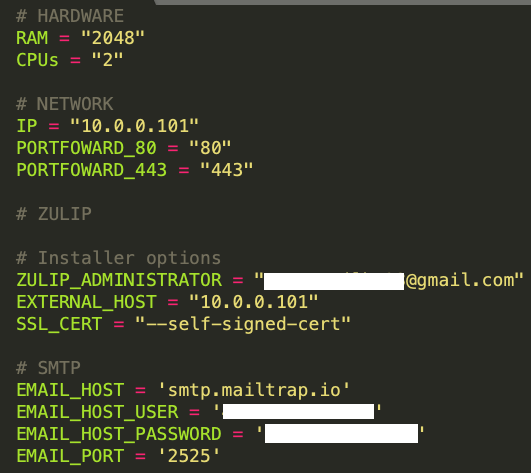
\includegraphics[scale=0.6]{automatizacao.png}
	\caption{Variáveis de instalação e configuração.}
	\label{img:pag}
\end{figure}
\chapter{Pontos críticos}

Analisando a arquitetura da aplicação \textbf{zulip}, verifica-se que existem componentes não replicados, sendo que, do ponto de vista do grupo, isso originará pontos críticos.\\

Deve ser aplicado a grande parte da arquitetura uma replicação, pois não se deve conter num sistema componentes, que em sua falta, causem a falha de todo o sistema. Deste modo, o componente do \textbf{servidor da base de dados} e o \textbf{aplicacional}, devem ser replicados para tornar a aplicação \textbf{zulip} tolerante a faltas, bem como reduzir os congestionamentos destes servidores. Operações que façam acessos à base dados, ou apenas ao servidor aplicacional, estão dependetes destes componentes, sendo crucial a fiablidade dos mesmos.\\

Deste modo, sugere-se a extensão da base de dados a pelo menos dois servidores \textbf{PostgreSQL}, bem como o servidor aplicacional, denominado \textbf{Django}. \\

Do mesmo modo, o componente \textbf{NGINX} também deve ser replicado, pois o mesmo é responável pela comunicação entre o \textbf{Client} e o restante sistema, logo a sua replicação tornará o sistema tolerante à sua falta, bem como distribuirá os pedidos pelas replicas, reduzindo a sobrecarga num único componente deste tipo.

\chapter{Conclusão}

Assim, finalizada a primeira fase do projeto, conclui-se que todos os objetivos inicialmente propostos foram cumpridos, tais como, análise da arquitetura, os padrões de distribuição e comunicação, a configuração da aplicação e por fim os pontos críticos da mesma.\\

Em relação à arquitetura da aplicação \textbf{zulip} a equipa baseou-se na documentação do website oficial da aplicação, onde a mesma é explicada detalhadamente. \\

\textbf{FALAR SOBRE OS PADRÕES DE COMUNICAÇÃO}\\

Para uma melhor perceção da configuração da aplicação a equipa decidiu instalar a mesma usando o \textbf{Vagrant}, e apresentar todos os passos neste relatório, tal como se pode verificar, com o objetivo de clarificar todos os processos da instalação. \\

Por fim, e não menos importante a análise dos pontos críticos da aplicação passou por uma análise da arquitetura da mesma e identifcar possíveis problemas. Os principais problemas encontrados foram a não tolerância a faltas do sistema e possíveis congestionamentos de servidores, quer da base de dados, bem como do servidor aplicacional.

\end{document}
